%%%%%%%%%%%%%%%%%%%%%%%%%%%%%%%%%%%%%%%%%%%%%%%%%%%%%%%%%%%%%%%%%%%%%%%%%%
%% Review Volume (last updated on 2014/03/05)                           %%
%% Trim Size: 9.61in x 6.69in                                           %%
%% Text Area: 8in (include runningheads) x 5in                          %%
%% Main Text: 10 on 13pt                                                %%
%% For support: Yolande Koh, <ykoh@wspc.com.sg>                         %%
%%              D. Rajesh Babu, <rajesh@wspc.com.sg>                    %%
%%%%%%%%%%%%%%%%%%%%%%%%%%%%%%%%%%%%%%%%%%%%%%%%%%%%%%%%%%%%%%%%%%%%%%%%%%
%%
%\documentclass[wsdraft]{ws-rv961x669} % to draw border line around text area
\documentclass{ws-rv961x669}
\usepackage{ws-rv-van}     % numbered citation/references (default)
\usepackage{ws-rv-thm}     % comment this line when `amsthm / theorem / ntheorem` package is used
\usepackage{subfigure}     % required only when side-by-side / subfigures are used
%\usepackage{ws-index}     % required only when multiple indexes are used
\makeindex
%\newindex{aindx}{adx}{and}{Author Index}       % author index
%\renewindex{default}{idx}{ind}{Subject Index}  % subject index

\begin{document}

\chapter[Spectrometers]{Spectrometer systems for radio astronomy}\label{spec_chap}

\author[D. Price, J. Hickish and D. Werthimer]{Danny C. Price, Jack Hickish and Dan Werthimer}

\address{Campbell Hall 339, UC Berkeley\\
Address goes here, \\
dancpr@berkeley.edu}

\begin{abstract}
This review gives an introduction to spectrometers and discusses their use within radio astronomy. While a variety of technologies are introduced, particular emphasis is given to digital systems, with details of current-generation implementations given as examples. Three different types of digital spectrometers are discussed: autocorrelation spectrometers (ACS), Fourier transform spectrometers (FTF), and polyphase filterbank spectrometers (PFB). The relative advantages and disadvantages of each technology are compared and contrasted. 

\end{abstract}

%\markright{Customized Running Head for Odd Page} % default is Chapter Title.

\body

\section{Introduction}\label{introduction}

A \emph{spectrometer} is a device used to record and measure the spectral content of signals, such as radio waves received from astronomical sources. Specifically, a spectrometer measures the power spectral density (PSD, commonly known as \emph{power spectrum}) of a signal. Analysis of spectral content can reveal details of radio sources, as well as properties of the intervening medium. For example, spectral line emission from simple molecules such as neutral hydrogen gives rise to narrowband radio signals (Fig.~1), while continuum emission from active galactic nuclei gives rise to wideband signals.


There are two main ways in which the PSD of a signal may be computed. The PSD, $S_{xx}$, of a waveform and its autocorrelation function,  $r_{xx}$, are related by the Wiener-Khinchin theorem. This theorem states that the relationship between a stationary (mean and variance do not change over time), ergodic (well-behaved over time) signal $x(t)$, its PSD, and its autocorrelation is given by
\begin{equation}
S_{xx}(\nu)=\int_{-\infty}^{\infty}r_{xx}(\tau)e^{-2\pi i\nu\tau}d\tau.
\label{eq:psd}
\end{equation}
where $\nu$ represents frequency, and $\tau$ represents a time delay or `lag'. The autocorrelation function is
\begin{equation}
r_{xx}(\tau)=\left\langle x(t)x(t-\tau)\right\rangle,
\end{equation}
where angled brackets refer to averaging over time. 

\begin{figure}
 \centering
 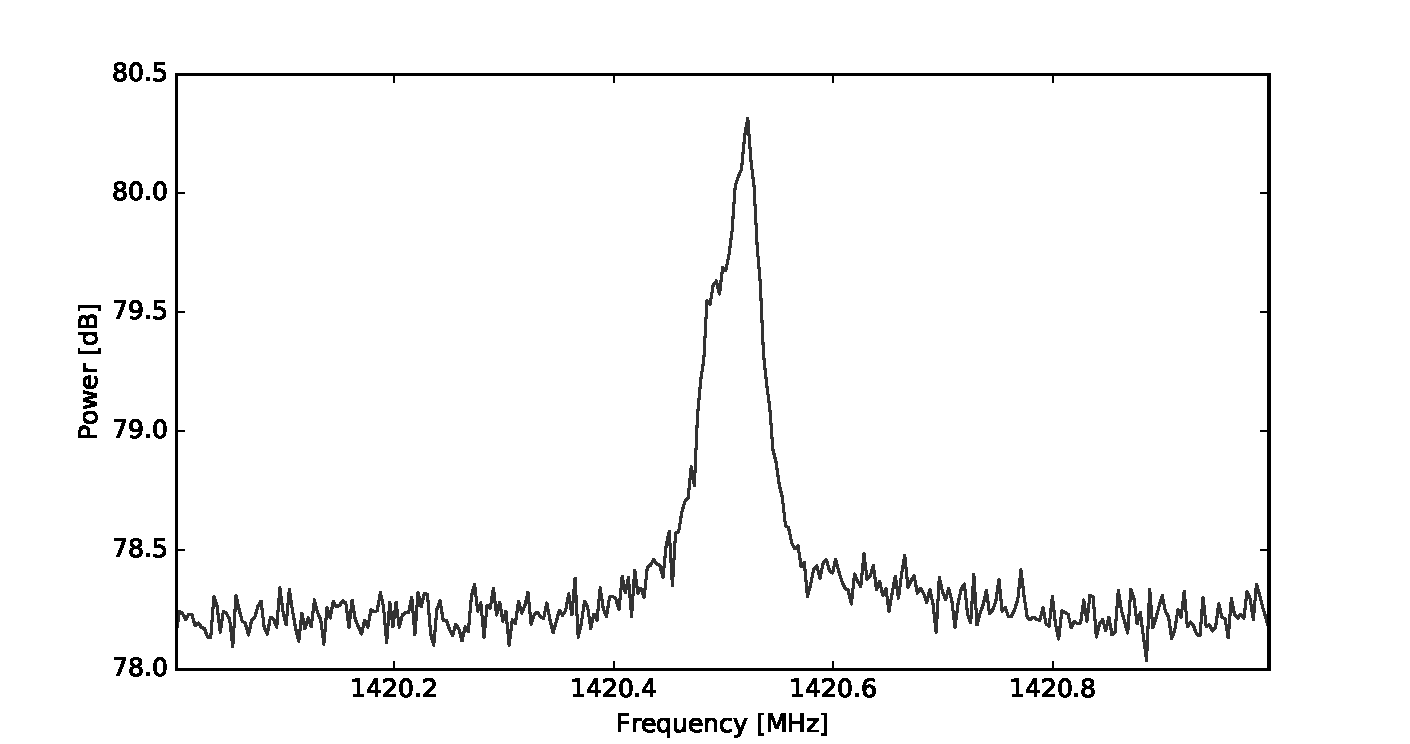
\includegraphics[width=\textwidth]{./figures/hydrogen.pdf}
 % analog-autocorr-crop.pdf: 0x0 pixel, 0dpi, nanxnan cm, bb=
 \label{fig:hydrogen}
 \caption{A galactic hydrogen 21-cm line emission profile, as measured using a digital spectrometer system on the Robert C. Byrd Greenbank Telescope in West Virginia.}
\end{figure}

Equation~\ref{eq:psd} shows that that the autocorrelation function is related to the PSD by a Fourier transform. In the discrete case, the relationship becomes
\begin{equation}
S_{xx}(k)=\sum_{k=-\infty}^{\infty}\left\langle x(n)x(n-k)\right\rangle e^{-2\pi ik\tau},\label{eq:discrete-wiener}
\end{equation}
which may be recognized as a discrete convolution. It follows from the convolution theorem that 
\begin{equation}
S_{xx}(k)=\left\langle \left|X(k)\right|^{2}\right\rangle ,\label{eq:discrete-pow}
\end{equation}
where $X(k)$ denotes the Discrete Fourier Transform (DFT) of $x(t)$:
\begin{equation}
X(k)=\sum_{n=0}^{N}x(n)e^{-2\pi ink/N}
\end{equation}

There are therefore two distinct classes of spectrometers: ones that approximate $S_{xx}(k)$ by firstly forming the autocorrelation, then taking a Fourier transform ala Eq.~\ref{eq:discrete-wiener}, and those that first convert into the frequency domain to form $X(k)$ before evaulating Eq.~\ref{eq:discrete-pow}.

\subsection{Analysis and synthesis filterbanks}

It is important to note the relationship between spectrometers, filters, and filterbanks. A \emph{filterbank} is simply an array of band-pass filters, designed to split an input signal into multiple components, or similarly, to combine multiple components. These are referred to as \emph{analysis} and \emph{synthesis} filterbanks, respectively. When applied to streaming data, a DFT can be considered an analysis filterbank, and an inverse DFT to be a synthesis filterbank; we return to this in XX. From this viewpoint, a spectrometer is simply an analysis filterbank, where the output of each filter is squared and averaged.

Analysis and synthesis filterbanks have many applications outside of astronomy, see [REF] for further discussion.

\subsection{Polarimetry}

Polarization is a key measurement within astronomy; textbooks such as \citet{BookTinbergenPolarim} are devoted to the subject.  Although most astrophysical radio emission is noise-like and thus inherently unpolarized, a number of radio sources -- such as pulsars and masers -- do emit polarized radiation, and effects such as Faraday rotation by a galaxy's magnetic field can yield polarized signals. Measuring polarization as a function of frequency can elucidate information about the source itself, and/or the medium between the source and observer. 

Most radio telescopes consist of a pair of orthogonal antennas, each of which is sensitive to a single polarization. 

The Stokes parameters are a set of quantities which fully describe the polarization state of an electromagnetic wave. These four parameters, $I$, $Q$, $U$ and $V$, are related to the amplitudes of perpendicular components of the electric field.
\begin{eqnarray}
E_{x} & = & e_{x}(t)cos(\omega t+\delta_{x})\\
E_{y} & = & e_{y}(t)cos(\omega t+\delta_{y})
\end{eqnarray}
by time averages of these electric field parameters:
\begin{eqnarray}
I & = & \left\langle E_{x}E_{x}^{*}+E_{y}E_{y}^{*}\right\rangle \\
Q & = & \left\langle E_{x}E_{x}^{*}-E_{y}E_{y}^{*}\right\rangle \\
U & = & \left\langle E_{x}E_{y}^{*}+E_{y}E_{x}^{*}\right\rangle \\
V & = & i\left\langle E_{x}E_{y}^{*}-E_{y}E_{x}^{*}\right\rangle 
\end{eqnarray}
The parameter $I$ is a measure of the total power in the wave, $Q$
and $U$ represent the linearly polarised components, and $V$ represents
the circularly polarised component. The Stokes parameters have the
dimensions of flux density, and they combine additively for independent
waves. See Figure~\ref{fig:Polarization} for a diagram.

\subsection{Radiometry and signal to noise}

Noise is inherent in any radio-frequency instrument. The system temperature, $T_{\rm{sys}}$, is a measure of the total noise of a telescope, including the noise contribution from the sky and antenna. To mitigate the effect of noise, one can take multiple measurements over bandwidth and time. The time it takes to reach a target root-mean-square noise temperature is then given by the ideal radiometer equation: 
\begin{equation}
\sigma_{T}=\frac{T_{sys}}{\sqrt{\mbox{2}n_{p}\Delta\nu t}},\label{eq:radiometer-eqn}
\end{equation}
where $n_{p}$ is the number of polarizations, and $\tau$ is integration time. The smallest detectable signal $T_{S}$ is given by $T_{S}=m\Delta T$, where $m$ is a threshold value, generally greater than or equal to 3. 

Spectrometers can increase the signal to noise ratio (SNR) of a radio telescope through both integration and channelization. Integration increases the SNR because signal increases linearly with integration whereas noise increases as the square root with integration. Thus, integrating longer by a factor of N will increase SNR by a factor of $\sqrt{N}$.

Channelization reduces the signal to noise of narrowband signals due to the fact that the noise power is divided equally across all spectral channels while the narrow band signal is confined to a comparatively smaller number of channels. For a sinusoidal signals, channelizing to N channels will reduce the per-channel noise power by a factor of N thereby increasing the per-channel SNR by a factor of N.


\section{Digital systems}

The first class are called lag-autocorrelators, or auto-correlation spectrometers (ACS). The second class are known as Fourier transform filterbanks (FTF).

There are two distinct classes of digital spectrometers: ones that approximate $S_{xx}(k)$ through numerical approximation to Equation~\ref{eq:discrete-wiener}, and those that evaulate Equation~\ref{eq:discrete-pow}. The first class are called lag-autocorrelators, or auto-correlation spectrometers (ACS). The second class are known as a discrete Fourier transform filterbanks (FTF).  


\subsection{Digital sampling}

As their name implies, \emph{analog to digital converters} (ADCs) convert analog signals into digital signals. The two main characteristics of an ADC are its sample rate and tbe number of bits per sample.

The ADC converts an analog voltage into a numeric quantity and then repeats the process. The numeric quantities are called \emph{samples}. The rate at which the ADC performs conversions is called the \emph{sample rate}. The sample rate, usually expressed in samples per second, determines the amount of bandwidth that can be unambiguoysly processed by an ADC. The Nyquist Theorem states that a band limited signal can be fully recovered when it is sampled at a rate that is twice the bandwidth. For example, a sample rate of 1 billion s

\subsubsection{Quantization efficiency}

Van Vleck and Non-Linearities

\subsubsection{Dynamic range}

\subsubsection{Interleaving}

\subsection{Windowing functions}

\begin{figure}
 \centering
 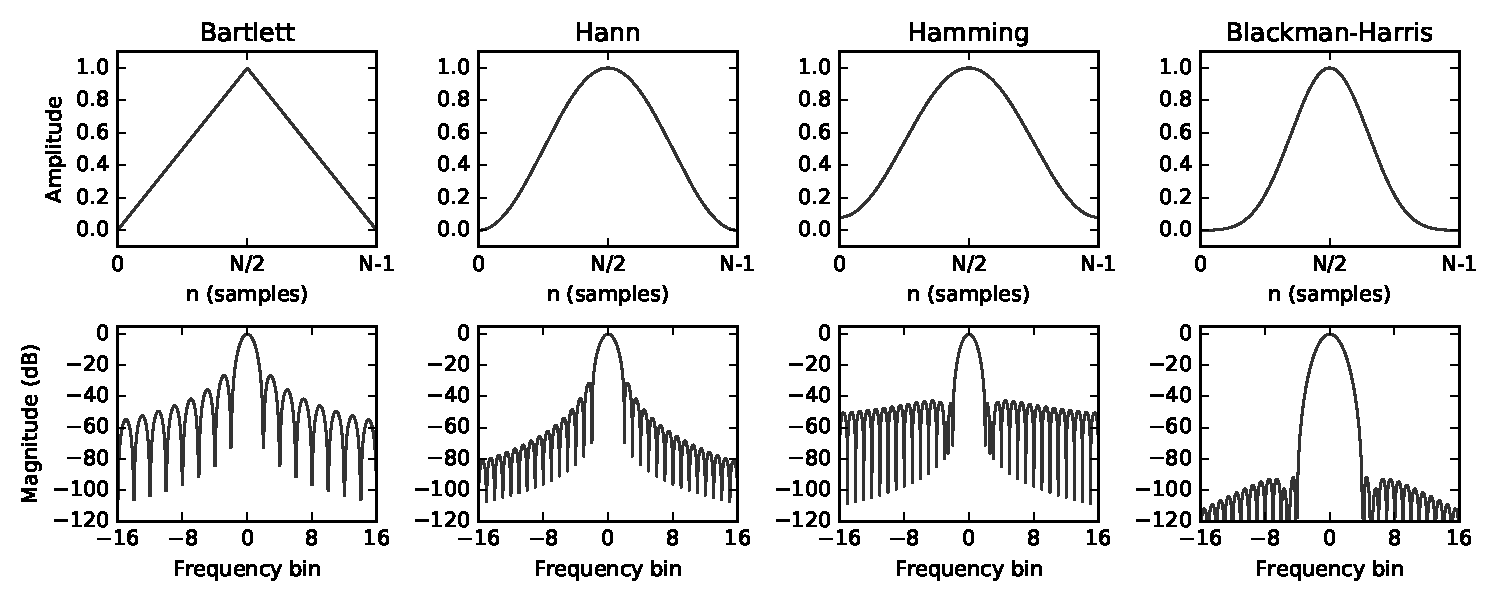
\includegraphics[width=\textwidth]{./figures/window_fns}
 \label{fig:window_fns}
 \caption{Four common windowing functions ($w(n)$, top) and their corresponding squared Fourier transforms ($|W(k)|^2$, bottom). Outside of the range [0, $N-1$], the function $w(n)=0$ for all windows.}
\end{figure}

\begin{table}
	\caption{Some common weighting functions used in FIR filter design. Note that in this table, coefficients have been rounded to four significant digits. \label{tab:adc}}
	\begin{tabular}{l l }
	\hline
	Weighting function      & $w(n)$                        			\\
	\hline
	\hline
	Uniform  (rectangular)   &  1                           			\\
	Bartlett (triangular)    &  $1 - (|n| / (N-1)$               	\\
	\hline
	\emph{General form:}    & $a_0 - a_1~cos(\frac{2\pi n}{N-1})$ \\
	Hann                     & $a_0=0.50 \quad a_1 = 0.50$ 	\\
	Hamming             & $ a_0 = 0.54 \quad a_1 = 0.46$   	\\
	\hline
	
	 \emph{General form:} &$a_0 - a_1~cos(\frac{2\pi n}{N-1}) + a_2~cos(\frac{4\pi n}{N-1}) -
	 					   a_3~cos(\frac{6\pi n}{N-1}) $	 \\
	 Nutall          & $a_0=0.3558\quad a_1=0.4874\quad a_2=0.1442\quad a_3=0.0126$ \\
	 Blackman-Nutall & $a_0=0.3636\quad a_1=0.4892\quad a_2=0.1366\quad a_3=0.0106$ \\
	 Blackman-Harris & $a_0=0.3588\quad a_1=0.4883\quad a_2=0.1413\quad a_3=0.0117$ \\
	\hline
	\end{tabular}

\end{table}

The spectral response of an FTF spectrometer can be improved by windowing the data before performing the DFT; in ACS architectures a windowing function may be applied after the autocorrelation step. An in-depth discussion of windowing functions is given in \citet{SvenGade1987}. 

For filterbanks, the Hamming and Hann windows are commonly applied windowing functions. The Hamming window has coefficients given by
\begin{equation}
w(n)=\mbox{0.54}-\mbox{0.46}cos\left(\frac{\mbox{2}\pi n}{N-1}\right),
\end{equation}
which are optimized to minimize the level of the first sidelobe. These coefficients are similar to those of the Hann window%
\footnote{Named after Julius von Hann, but often erroneously referred to as
`Hanning'.%
}:
\begin{equation}
w(n)=\mbox{0.5}(\mbox{1}-cos\left(\frac{\mbox{2}\pi n}{N-1}\right),
\end{equation}
which offers faster sidelobe rolloff, but a higher first-sidelobe
level. 

A more dramatic improvement may be achieved by using an lowpass filter frontend before the DFT \citep{Bellanger:1976p7898}, to form what is known as a polyphase filterbank (PFB). This approach is detailed further in the following section. Figure~\ref{fig:PFB-num-taps} compares the spectral response of a standard DFT (`vanilla'), Hamming windowed DFT, and polyphase filterbank, for a single channel. An example showing a 16-channel, 4-tap Hamming window-based polyphase filterbank is shown in Figure~\ref{fig:PFB-8tap-16ch-example}.

A filterbank is simply a collection of filters, a simple example being a highpass and lowpass filter pair. I discuss here filterbanks where each filter has identical passband characteristics and evenly spaced central frequencies, such as the 16 channel filterbank shown in Figure~\ref{fig:PFB-8tap-16ch-example}. This equally spaced form is the most commonly implemented for radio astronomy applications. 

This section begins with a short overview of digital filtering techniques; I refer the reader unfamiliar with digital signal processing to the excellent \citet{bookLyonsDSP} and \citet{BookSmithDSP}. A comprehensive overview of polyphase filters is given by \citet{Vaidyanathan:1990p6127}, and in Chapter~2 of \citet{BookHarrisMultirateDSP}; I will give a brief introduction here. In the diagrams that follow, the symbol $\otimes$ denotes multiplication of time samples, and $\oplus$ denotes addition. The symbol $z^{-n}$ is used to denote a time delay of \emph{n} units, and the symbol $\downarrow D$ is used for downsampling by a factor \emph{D} and $\uparrow U$ for upsampling by a factor \emph{U}.



\subsection{Finite impulse response filters}

A finite impulse response (FIR) filter is the windowed moving average of an input sequence $x(t)$. An FIR filter computes the sum 
\begin{equation} 
y(t)=\sum_{k=0}^{K-1}h(k)x(t-k),\label{eq:FIR-filter}
\end{equation}
where $y(n)$ is the output sequence, and $h(k)$ is a set of $K$ coefficients used for weighting. The upper summation bound, \emph{K}, is called the number of taps.\emph{ }A streaming implementation of an FIR filter is shown in Figure~\ref{fig:N-tap-FIR-filter}.

If we downsample after an FIR by $\downarrow D$, we only keep the outputs $t=mD$, $m\in\mathbb{Z}^{+}$. A $\downarrow D$ downsampled filter will alias spectra centred at any multiple of the output sample rate to baseband. In such cases it is more efficient to only compute the terms we wish to keep: 
\begin{equation}
y(mD)=\sum_{k=0}^{K-1}h(k)x(mD-k).\label{eq:FIR-filter-decimated}
\end{equation}
One way we can accomplish this is to use a polyphase decimating filter, which is discussed below. 


\subsection{Polyphase FIR filters}

A common technique in DSP is to decompose an input sequence $x(t)$ into a set
\begin{equation}
\mathbb{P}=\begin{Bmatrix}x_{k}(t) & k\in(0,P-1)\end{Bmatrix}
\end{equation}
of $P$ sub-sequences, $x_{k}(t)$, each of which is given by 
\begin{equation}
x_{k}(t)=(\downarrow P)(z^{-k})x(t).
\end{equation}
This is known as polyphase decomposition. Even and odd decomposition
of the signal $x(t)$ is achieved when $P=\mbox{2}$:
\begin{eqnarray}
x_{0}(t) & = & \left\{ x(0),x(2),x(4),...\right\} \\
x_{1}(t) & = & \left\{ x(1),x(3),x(5),...\right\} .
\end{eqnarray}
More generally, an input stream may be decomposed into $P$ different `phases'.

Polyphase filter structures are often more efficient than standard finite impulse response filters when used in sample rate conversion. A $\downarrow P$ decimating FIR filter of length $K=MP$ can be constructed from $P$ discrete FIR filter `branches', each acting upon a different phase; that is
\begin{equation}
y(t)=\sum_{p=0}^{P-1}\sum_{m=0}^{M-1}h_{p}(m)x_{p}(t-m),\label{eq:FIR-polyphase-filter}
\end{equation}
This is known as a decimating polyphase filter. For example, a $P=\mbox{4}$ branch polyphase filter with $M=\mbox{7}$ taps per sub-filter would compute the sum
\begin{eqnarray}
y(t) & = & \sum_{m=0}^{7}h_{0}(m)x_{0}(t-m)+\sum_{m=0}^{7}h_{1}(m)x_{1}(t-m)\nonumber \\
 & + & \sum_{m=0}^{7}h_{2}(m)x_{2}(t-m)+\sum_{m=0}^{7}h_{3}(m)x_{3}(t-m),
\end{eqnarray}
and has an output equivalent to a $\mbox{4}\times\mbox{7}=\mbox{28}$ tap standard FIR filter with 4:1 downsampling. 

Decimating polyphase filter structures are more efficient than standard FIR filter based downsampling techniques. If $\downarrow D$ downsampling occurs after the moving average of Equation~\ref{eq:FIR-filter}, we compute \emph{D} sums, but keep only 1 in \emph{D} of these. This is inefficient. In comparison, Equation~\ref{eq:FIR-polyphase-filter} only computes the output values that are of interest. A comparison of two decimating filters is shown in Figure~\ref{fig:polyphase-filters}. Figure~\ref{fig:polyphase-filterb} is a polyphase type structure, but decimation occurs after summation. Conversely, Figure~\ref{fig:polyphase-filterb} shows a more efficient implentation where decimation occurs before summation. By the noble identities (see \citep{Vaidyanathan:1990p6127}), the output of this second filter is identical to that in Figure~\ref{fig:polyphase-filterb}.


\subsection{The Fast Fourier Transform}

* Radix 2 stuff

\section{Digital spectrometers}

The first digital spectrometer used for radio astronomy was developed by \citet{Weinreb:1963p10042}. This 1-bit ACS was used to observe the 18-cm wavelength hydroxyl (OH) absorption line in the spectrum of Cassiopeia A, providing the first evidence of OH in the interstellar medium \citep{Weinreb:1963p9992}. The first reference to FTF spectrometers for radio astronomy can be found in \citet{Chikada:1987p10044}; however FTF spectrometers did not enjoy widespread adoption until much later. This is due to implementation issues, such as increased data output rates as compared to ACS implementations; see \citet{Bunton2000}, for a discussion of these issues.


\subsection{Performance characteristics}

* Spectral leakage
* Scalloping loss
* Time resolution
* Dynamic range

\subsection{Autocorrelation spectrometers}

Digital autocorrelators implement the autocorrelators delay-and-multiply circuitry using digital delays -- shift registers -- and digital multiplier cores to compute signal products. As a result, digital correlators can have much more predictable performance than their analog counterparts whose processing is subject to small errors in delay line lengths and other subtle analog effects. In contrast, provided signals in a digital autocorrelator can be digitised with adequate signal-to-noise and linearity the downstream autocorrelation computation can be regarded as possesing perfect precision.

Digital systems are usually prefered when the bandwidth to be processed is within the capabilities of commercially available ADC chips. However, if the number of frequency channels desired is large an FFT-based spectrometer may be preferable to an autocorrelation system. FFT spectrometers are described more fully in Section \ref{digital-fft} and can be inplemented with vastly lower computational overhead, at the cost of increased design complexity.

\subsection{Fourier transform spectrometers}

A time-domain signal $v(t)$ may be spectrally decomposed using a Fourier Transform, defined by:

\begin{equation}
 \label{ft}
 V(f) = \int_{-\infty}^{\infty} v(t) e^{-2\pi i f} \,\mathrm{d}t\, .
\end{equation}

In a digital system, where an input has been discretely sampled $N$ times with values $v_n$ the Fourier Transform may be reduced to its discrete form: 

\begin{equation}
 \label{dft}
 V_f = \sum_{n = 0}^{N-1} v_n e^{\frac{-2\pi i f n}{N}} \hspace{1cm} f = [0, N-1]\,.
\end{equation}

Equation \ref{dft} may be thought of as the mixing of the input signal with a bank of oscillators, followed by an averaging with a square window function. In effect, this is a simple filterbank.

In general, computing Equation \ref{dft} for each value of $f$ requires $N$ multiplications, and $N$ additions. Since $f$ can take $N$ independent values itself, the total cost of implementing a DFT filterbank is $N^2$ operations per transform. If one transform is computed for every $N$ samples digitized, then the computation rate is of order $F_sN$ operations each second, where $F_s$ is the sampling rate.

In the case that samples $v_n$ are regularly spaced in time (which they almost invariably are) the Fast Fourier Transform (FFT, \cite{Cooley1965}) algorithm allows Equation \ref{dft} to be evaluated in $O(N\log_2(N))$ operations, or $F_s\log_2(N)$ if performed every $N$ samples. With computational savings of order $N / \log2{N}$ the FFT is an extraordinarily powerful algorithm, which is used heavily throughout radio astronomy. For a spectrometer of $~10^4$ channels, the FFT algorithm requires approximately $0.1\%$ as many operations as an autocorrelation spectrometer.







\subsection{Polyphase filterbanks}

In comparison to both ACS and FTF architectures, polyphase filterbanks offer vastly improved interchannel isolation. For radio astronomy
purposes, high interchannel isolation is important so that spectral features are not smeared out, and so the spectrometer is more resilient to the high levels of radio frequency interference (RFI) emitted from terrestrial sources. Polyphase filterbanks are therefore the best candidate for radio astronomy spectrometers, if computationally affordable.

A computationally efficient filterbank with high interchannel isolation can be constructed from an FFT preceded by a prototype polyphase FIR filter frontend. Such an implementation exploits the fact that a lowpass filter with coefficients $h(k)$, can be converted into a quadrature (complex) bandpass filter with central frequency $\omega_{k}$ by multiplying the coefficients by $e^{i\omega_{k}t}$ . That is, 
\begin{equation}
h_{bpf}(k)=h(k)e^{i\omega_{k}t}.\label{eq:lowpass-to-bandpass}
\end{equation}
Now, suppose we have a decimating lowpass polyphase filter, such as that in Figure~\ref{fig:polyphase-filterb}. The output of each branch
is 
\begin{equation}
y_{p}(t)=\sum_{m=0}^{M-1}h_{p}(m)x_{p}(t-m),
\end{equation}
where $h_{p}(m)$ are coefficients from our prototype lowpass filter. If we follow this by a DFT, as in Figure~\ref{fig:polyphase-filterd}, we then have 
\begin{eqnarray}
Y(k) & = & \sum_{p=0}^{P-1}y_{p}(t)e^{-2\pi ikp/P}\\
 & = & \sum_{p=0}^{P-1}\sum_{m=0}^{M-1}h_{p}(m)e^{-2\pi ikp/P}x_{p}(t-m).
\end{eqnarray}
Comparing this form to Equation~\ref{eq:FIR-filter-decimated} and Equation~\ref{eq:lowpass-to-bandpass}, we recognise that the output
of this structure --- Figure~\ref{fig:polyphase-filterd} --- is equivalent to a set of $\downarrow P$ downsampling polyphase filters:
\begin{equation}
\mathbb{F}=\begin{Bmatrix}h_{k}(m), & k\in(0,P-1)\end{Bmatrix}
\end{equation}
where the central frequency of each filter is shifted by an amount $\mbox{2}\pi ik/P$. For data sampled at the Nyquist rate $f_{s}$,
this filterbank consists of $N$ filters spanning $-f_{s}/\mbox{2}$ to $f_{s}/\mbox{2}$, with each filter separated by $f_{s}/\mbox{2}N$.
For real sampled data the negative frequencies contain no extra information, so they need not be computed. This leaves a a bank of $N/\mbox{2}$ filters, evenly spaced over a bandwidth $f_{s}/\mbox{2}$. This is the structure that I have implemented.

This polyphase filterbank (PFB) structure was first proposed by \citet{Bellanger:1976p7898}, and has been previously used in radio astronomy applications, see for example \citet{Zimmerman:1991p6933} and \citet{Parsons:2006p257}. The rest of this chapter discusses the implementation of a 8192 channel polyphase filterbank for radio astronomy, on Field Programmable Gate Array based digital hardware.

\begin{figure}
 \centering
 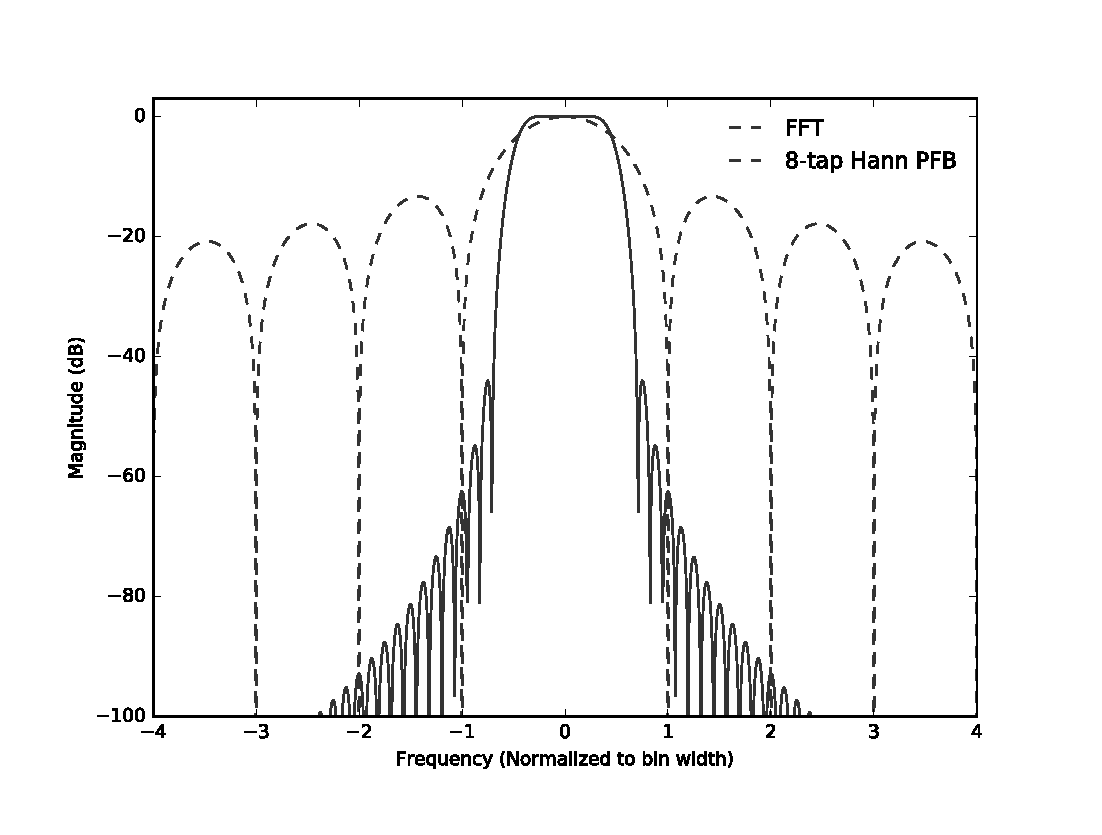
\includegraphics[width=\textwidth]{./figures/pfb_resp}
 \label{fig:pfb_response}
 \caption{Comparison of the filter response of a FFT spectrometer channel (dotted line) to an 8-tap, Hann-windowed PFB (solid line).}
\end{figure}

\begin{figure}
 \centering
 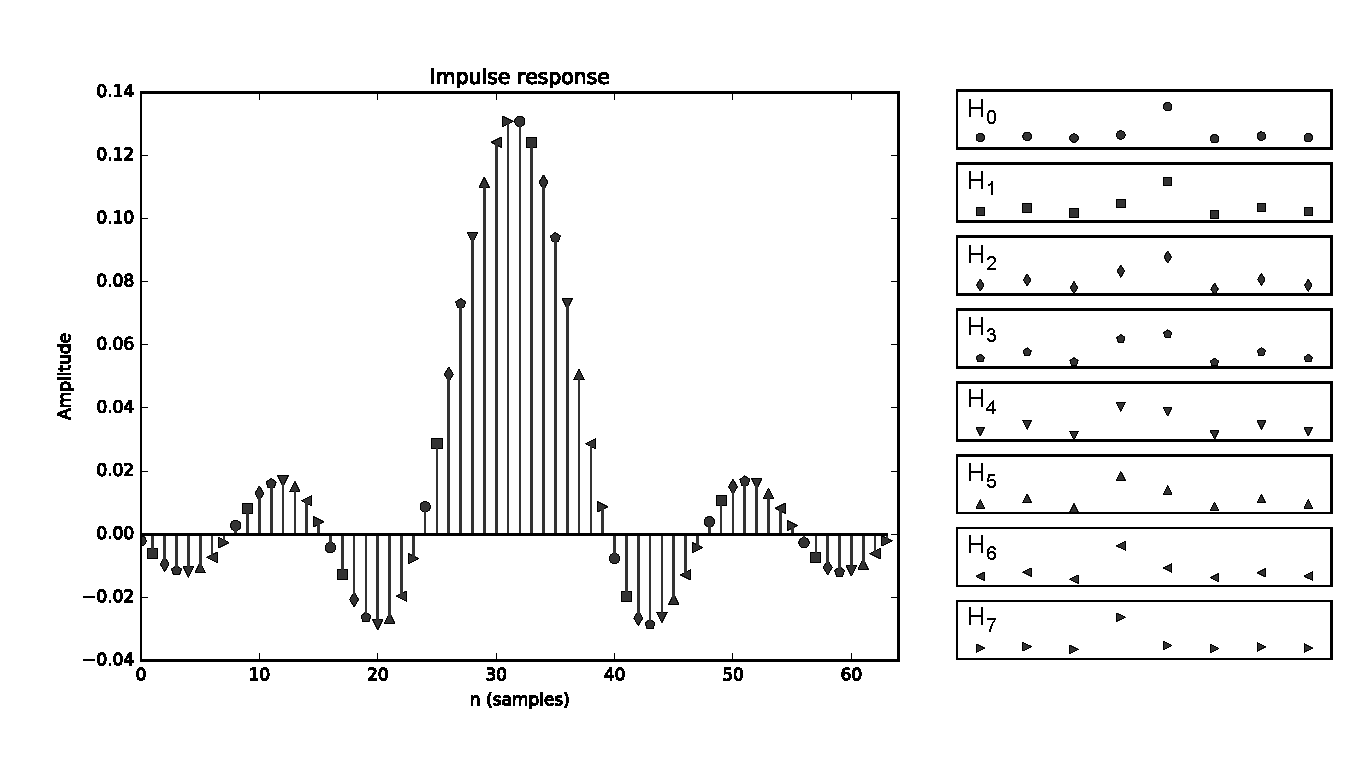
\includegraphics[width=\textwidth]{./figures/pfb_taps}
 \label{fig:pfb_taps}
 \caption{Example illustrating the polyphase decomposition of the coefficients h(k) of a 64-tap FIR filter (left) into 8 sub-filters (right). Each sub-filter has 8 taps; that is, P=8 and M=8. These sub-filters may be re-combined in a suitable polyphase filter structure to form a filter with an impulse response equal to the original FIR filter (left).}
\end{figure}

\begin{figure}
 \centering
 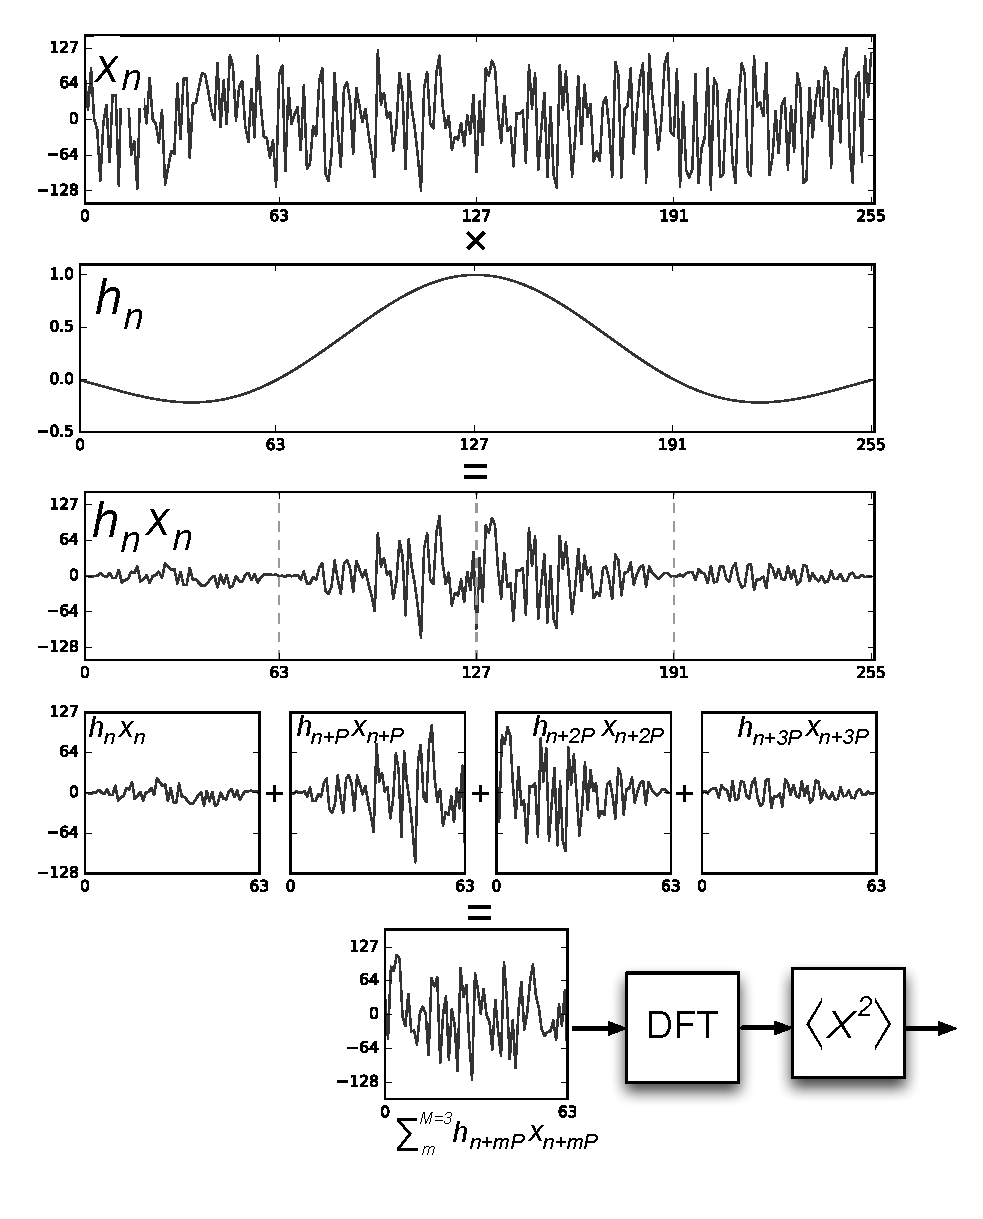
\includegraphics[width=\textwidth]{./figures/pfb_chart}
 \label{fig:pfb_chart}
 \caption{}
\end{figure}

\subsection{Implementation comparison}

ACS and FTF architectures differ in both their spectral response and the number of computations required to implement them. For regularly
sampled data, the Fast Fourier Transform (FFT) algorithm may be used to compute the DFT (see, for example, \citep{BookBrighamFFT}),
which reduces the number of computations required from $O(N^{2})$ for to $O(Nlog(N))$. In Chapter~4 of \citep{Taylor1999}, Romney
shows that the ratio of multiplies for the two architectures is 
\begin{equation}
R_{\frac{ACS}{FTF}}=\frac{n_{t}}{\mbox{2}log_{2}(n_{t})},
\end{equation}
where $n_{t}$ is the number of samples per FFT or lag correlation. So in general, FTF architectures require fewer computations than their equivalent ACS counterpart. Romney also shows that the spectral response of FTF and ACS architectures differ, with ACS architectures having a $sinc$ reponse, and FTF architectures posessing a $sinc^{2}$ response. The result is that interchannel isolation is better in FTF architectures (first sidelobe at $\sim-\mbox{13.6}$ dB), than in ACS architectures ($\sim-\mbox{6.8}$ dB). 

\subsection{Zoom modes}

\section{Alternative spectrometer implementations}

\subsection{Swept spectrometer}\label{swept-spectrometer}

\begin{figure}
 \centering
 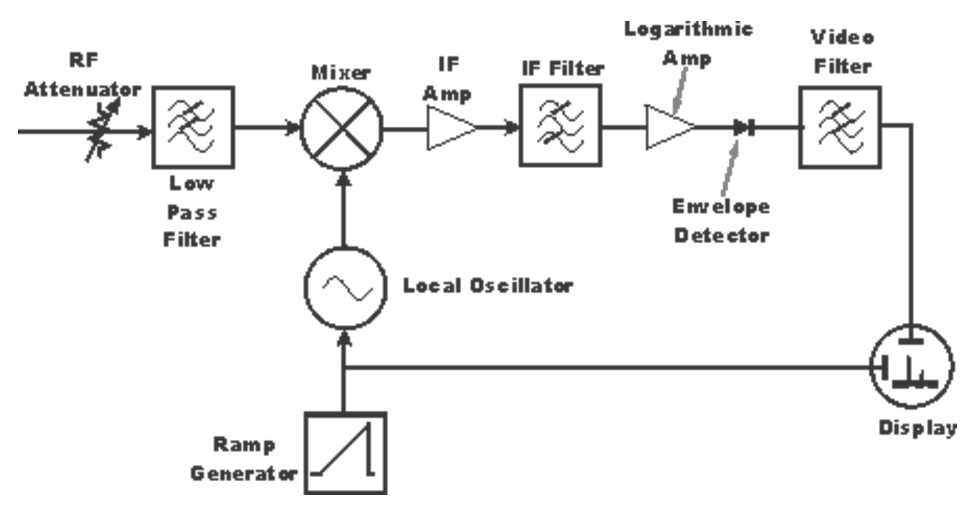
\includegraphics[width=\textwidth]{./figures/temp_spec_an_diagram}
 % analog-autocorr-crop.pdf: 0x0 pixel, 0dpi, nanxnan cm, bb=
 \label{fig:swept-an}
 \caption{Swept spectrum analyzer block diagram, need to remake. We can't use this image because a) it's low quality and b) it's not ours. \label{fig:swept}}
\end{figure}

A \emph{swept spectrometer} uses a variable oscillator with a heterodyne
circuit and a low pass filter (Fig.~\ref{fig:swept}). The oscillator is typically varied, i.e.~swept, through a range of desired frequencies. As it is swept through the desired frequency range, the power of the low pass filter's output is measured and recorded. Most analog spectrum analyzers operate in this manner.

An advantage of swept spectrometers is that they can operate over large RF bandwidths. However, as only a fraction of the band is detected at any one time, less integration time is available per frequency channel. For a swept spectrometer with $N$ channels with a sweep time of $t_{\rm{sweep}}$, the integration time available per channel is $t_{\rm{sweep}}/N$. It follows that  the RMS noise per channel is $\sqrt{N}$ higher than an equivalent filterbank spectrometer covering the entire RF bandwidth. As such, swept spectrometers are best suited for cases where signals of interest are strong and wideband. 

\subsection{Analog Filter Bank}\label{analog-filter-bank}

An \emph{analog filter bank} is just what its name implies: a bank (or collection) of analog filters. The analog filters are designed to pass through different ranges of frequencies. The power of the analog filters' output is measured and recorded. By creating a bank of filters with adjacent and non-overlapping passband frequencies one can get a complete picture of the input signal's spectrum.

\subsection{Analog autocorrelators}\label{autocorrelators}
The power spectrum of a signal, $S(f)$,  is related to the signal's autocorrelation function, $R(\tau)$, over a range of time lags, $\tau$, by Fourier transform:
\begin{equation}
\label{spec-from-autocorr}
 S(f) = \int_{-\infty}^{\infty} R(\tau)e^{-2\pi i \tau f} \,\mathrm{d}\tau \,.
\end{equation}

Thus, if one can build a device to measure the autocorrelation function of a signal of interest, it is straightforward to obtain the signal's power spectrum.
When integrated over a time $T$, the autocorrelation of a signal specified by the time-varying voltage $v(t)$ is defined by 

\begin{equation}
\label{autocorr}
 R(\tau) = \frac{1}{2T} \int_{-T}^{T} v(t)v(t+\tau) \,\mathrm{d}t \,.
\end{equation}

Since $v(t)$ is a real-valued function $R(\tau)$ is necessarily symmetric about positive and negative lags, so only one half need be measured. Furthermore, the symmetry of $R(\tau)$ means that the only contributions to $S(f)$ are from the even parts of the complex exponential in Equation \ref{spec-from-autocorr}. The computation of the power spectrum can then be reduced to:

\begin{equation}
\label{spec-from-autocorr-reduced}
 S(f) = 2\int_{0}^{\infty} R(\tau)\cos{(2\pi \tau f)} \,\mathrm{d}\tau \,.
\end{equation}

Regardless of autocorrelator implementation, it is invariably the case that Equation \ref{spec-from-autocorr-reduced} is computed for only a discrete range of delays, $\tau$. In much the same way as the sampling rate of an analog signal determines how much bandwidth can be processed unambiguously (see Section \ref{analog-to-digital-converters}) the spacing of lags in an autocorrelator determines how much bandwidth it can process without aliasing occuring. In the case of an autocorrelator the Nyquist criterion is satisfied when there are two taps per wave period at the highest frequency (shortest wavelength) signal of interest. 


\subsubsection{Analog Autocorrelators}\label{analog-autocorrelators}

Analog correlators are those that measure the autocorrelation function (Equation \ref{autocorr}) using analog circuitry to implement multipliers and propagation times through carefully constructed delay lines to implement the desired tap delays.
A typical schematic of an analog autocorrelator is shown in Figure \ref{fig:analog-autocorr}. Here, outputs of each correlator tap are digitized after a small amount of time-averaging. Further averaging can take place digitally before computation of the power spectrum via cosine transform. Details of specific scientific deployments of analog autocorrelation spectrometers can be found in \cite{Erickson2007} and \cite{Harris1998}.

The main advantage of the analog autocorrelator over its digital counterpart (see Section \ref{digital-autocorrelators}) is that digitization need only take place at a rate commensurate with the averaging period of the correlator, rather than the bandwidth of the input signals. For this reason, analog autocorrelation spectrometers are usually seen in systems that have instantaneous bandwidths of many gigahertz which cannot be readily digitized by commercially available ADCs.


\begin{figure}
 \centering
 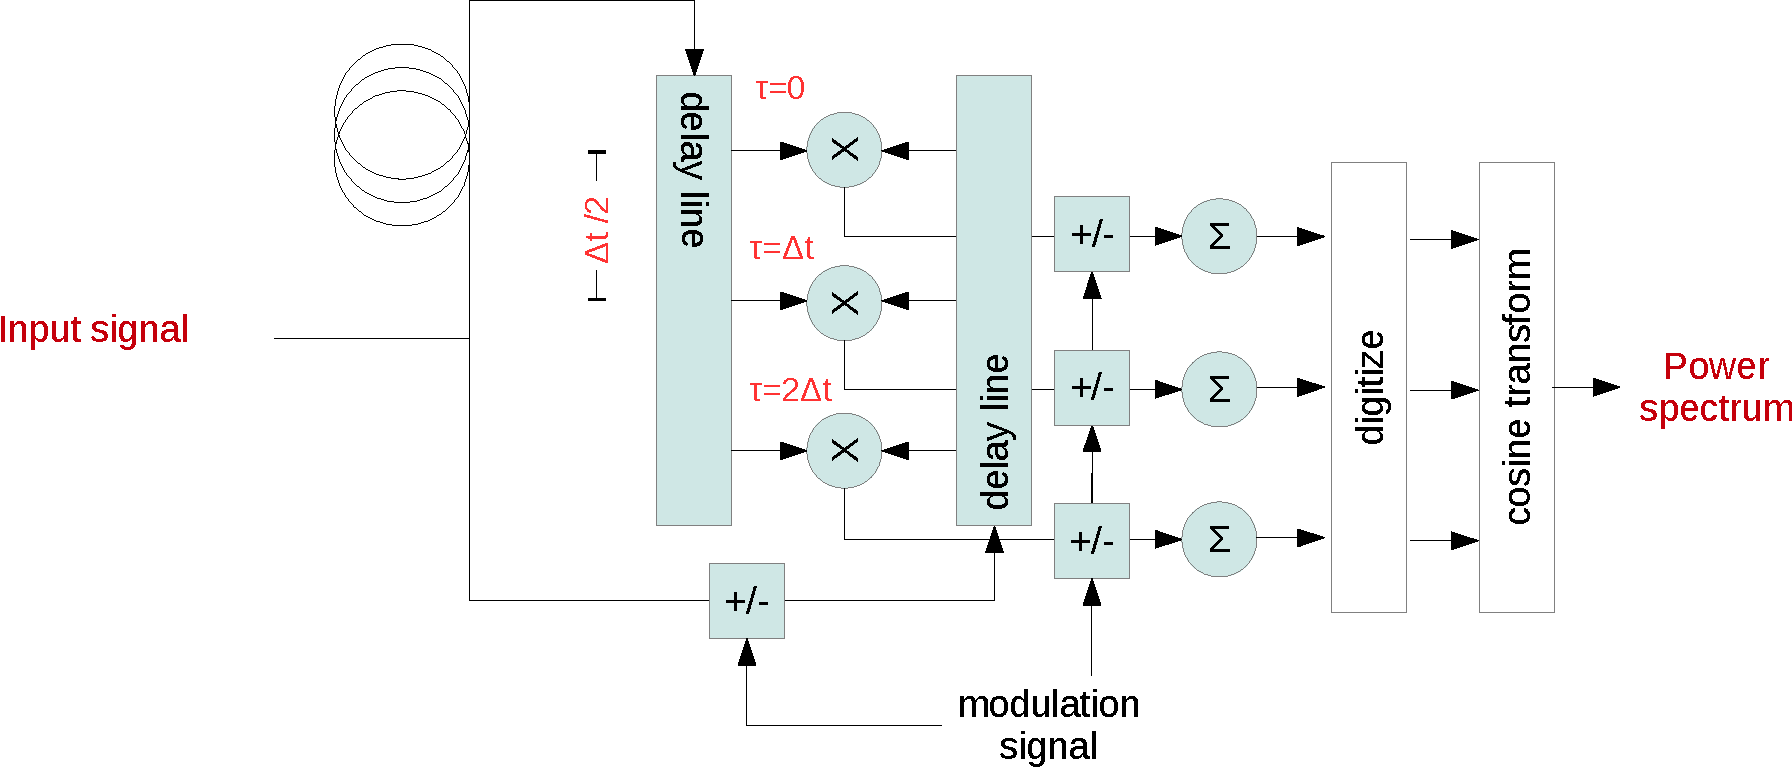
\includegraphics[width=\textwidth]{./figures/analog-autocorr-crop.pdf}
 % analog-autocorr-crop.pdf: 0x0 pixel, 0dpi, nanxnan cm, bb=
 \label{fig:analog-autocorr}
 \caption{An example implementation of an analog autocorrelator. The input signal is circulated in opposite directions down a pair of delay lines. The signal is tapped on each delay line at points separated by propagation delays of $\frac{\Delta t}{2}$. Each tap computes an element of the correlation with lag $\tau=n\Delta t$.}
\end{figure}

Figure \ref{fig:analog-autocorr} also indicates circuitry for modulating the input and outputs of the correlator. Such switching can serve multiple purposes. Firstly, it is sometimes advantageous for cost or performance reasons to prefer square-law diode detectors in favour of multiplication circuitry. These have a respose to inputs $v_1$ and $v_2$ of
\begin{equation}
 v_1^2 + v_2^2 + 2v_1v_2 \, .
\end{equation}

The last term is equal to the output of a multiplier, while the first two terms represent unwanted parts of the diode response. These unwanted terms can be eliminated by periodically alternating the sign of one of the inputs $v_1$ or $v_2$. This has no effect on the unwanted terms, but causes the last term to alternate sign. If, prior to time averaging, the sign of the diode output is flipped synchronously with the input then the unwanted terms will, up to a noise contribution, be removed.

In general, the principal of modulating the desired part of a signal and then synchronously demodulating to cancel out unwanted contributions can be used to surpress a variety of unwanted effects in radio receivers, such as gain variation and cross-coupling. An operating telescope may have multiple such switching systems operating concurrantly at different frequencies targetting different effects. See, for example, \cite{Erickson2007}. 

\subsection{Acousto-Optic}\label{acousto-optic}

\subsection{Hybrid Analog-Digital}\label{hybrid-analog-digital}




\section{Spectrometer design considerations}

\subsection{Technology choice}
What's Available Commercially

\begin{itemize}
	\item GPU
    \item CPU
    \item ASIC
    \item FPGA
    \item Heterogeneous	
\end{itemize}


\section{Examples}

\subsection{CASPER}

* Fast Readout Spectrometers for Pulsar Timing and Search

* Multibeam spectrometer systems

\section{Conclusions}

Polyphase filterbanks have attractive characteristics for radio astronomy applications. They offer excellent interchannel isolation and can be implemented using efficient FFT based structures. Field Programmable Gate Arrays are a viable platform on which to implement wide bandwidth polyphase filterbank spectrometers. I have implemented such a spectrometer using the Xilinx toolflow and CASPER block libraries. In this chapter I detailed the implementation and presented results on its performance.

\section{Acknowledgements}

The authors thank members of the CASPER collaboration for sharing their extensive knowledge with the wider community. D. Price thanks J. Moran for thorough discussion and debate on the virtues of polyphase filterbanks. 

\bibliographystyle{plain}
\bibliography{spectrometers,references}

\end{document}
